\documentclass[11pt, oneside]{amsart}
\usepackage{geometry}
\geometry{a4paper,top=1in,bottom=1in}
\usepackage[parfill]{parskip}
\usepackage{graphicx}
\usepackage{amssymb}
\pagestyle{empty}
\title{Tages Anzeiger math problems}

\begin{document}
\maketitle

The Zürich daily {\em Tages Anzeiger} has a weekly math column. Here are some
problems (translated from German to English) and my solutions.

\section{2024-05-02: Overlapping squares}

Three squares with the given side lenghts overlap as follows:

\begin{figure}[!h] 
    \centering
    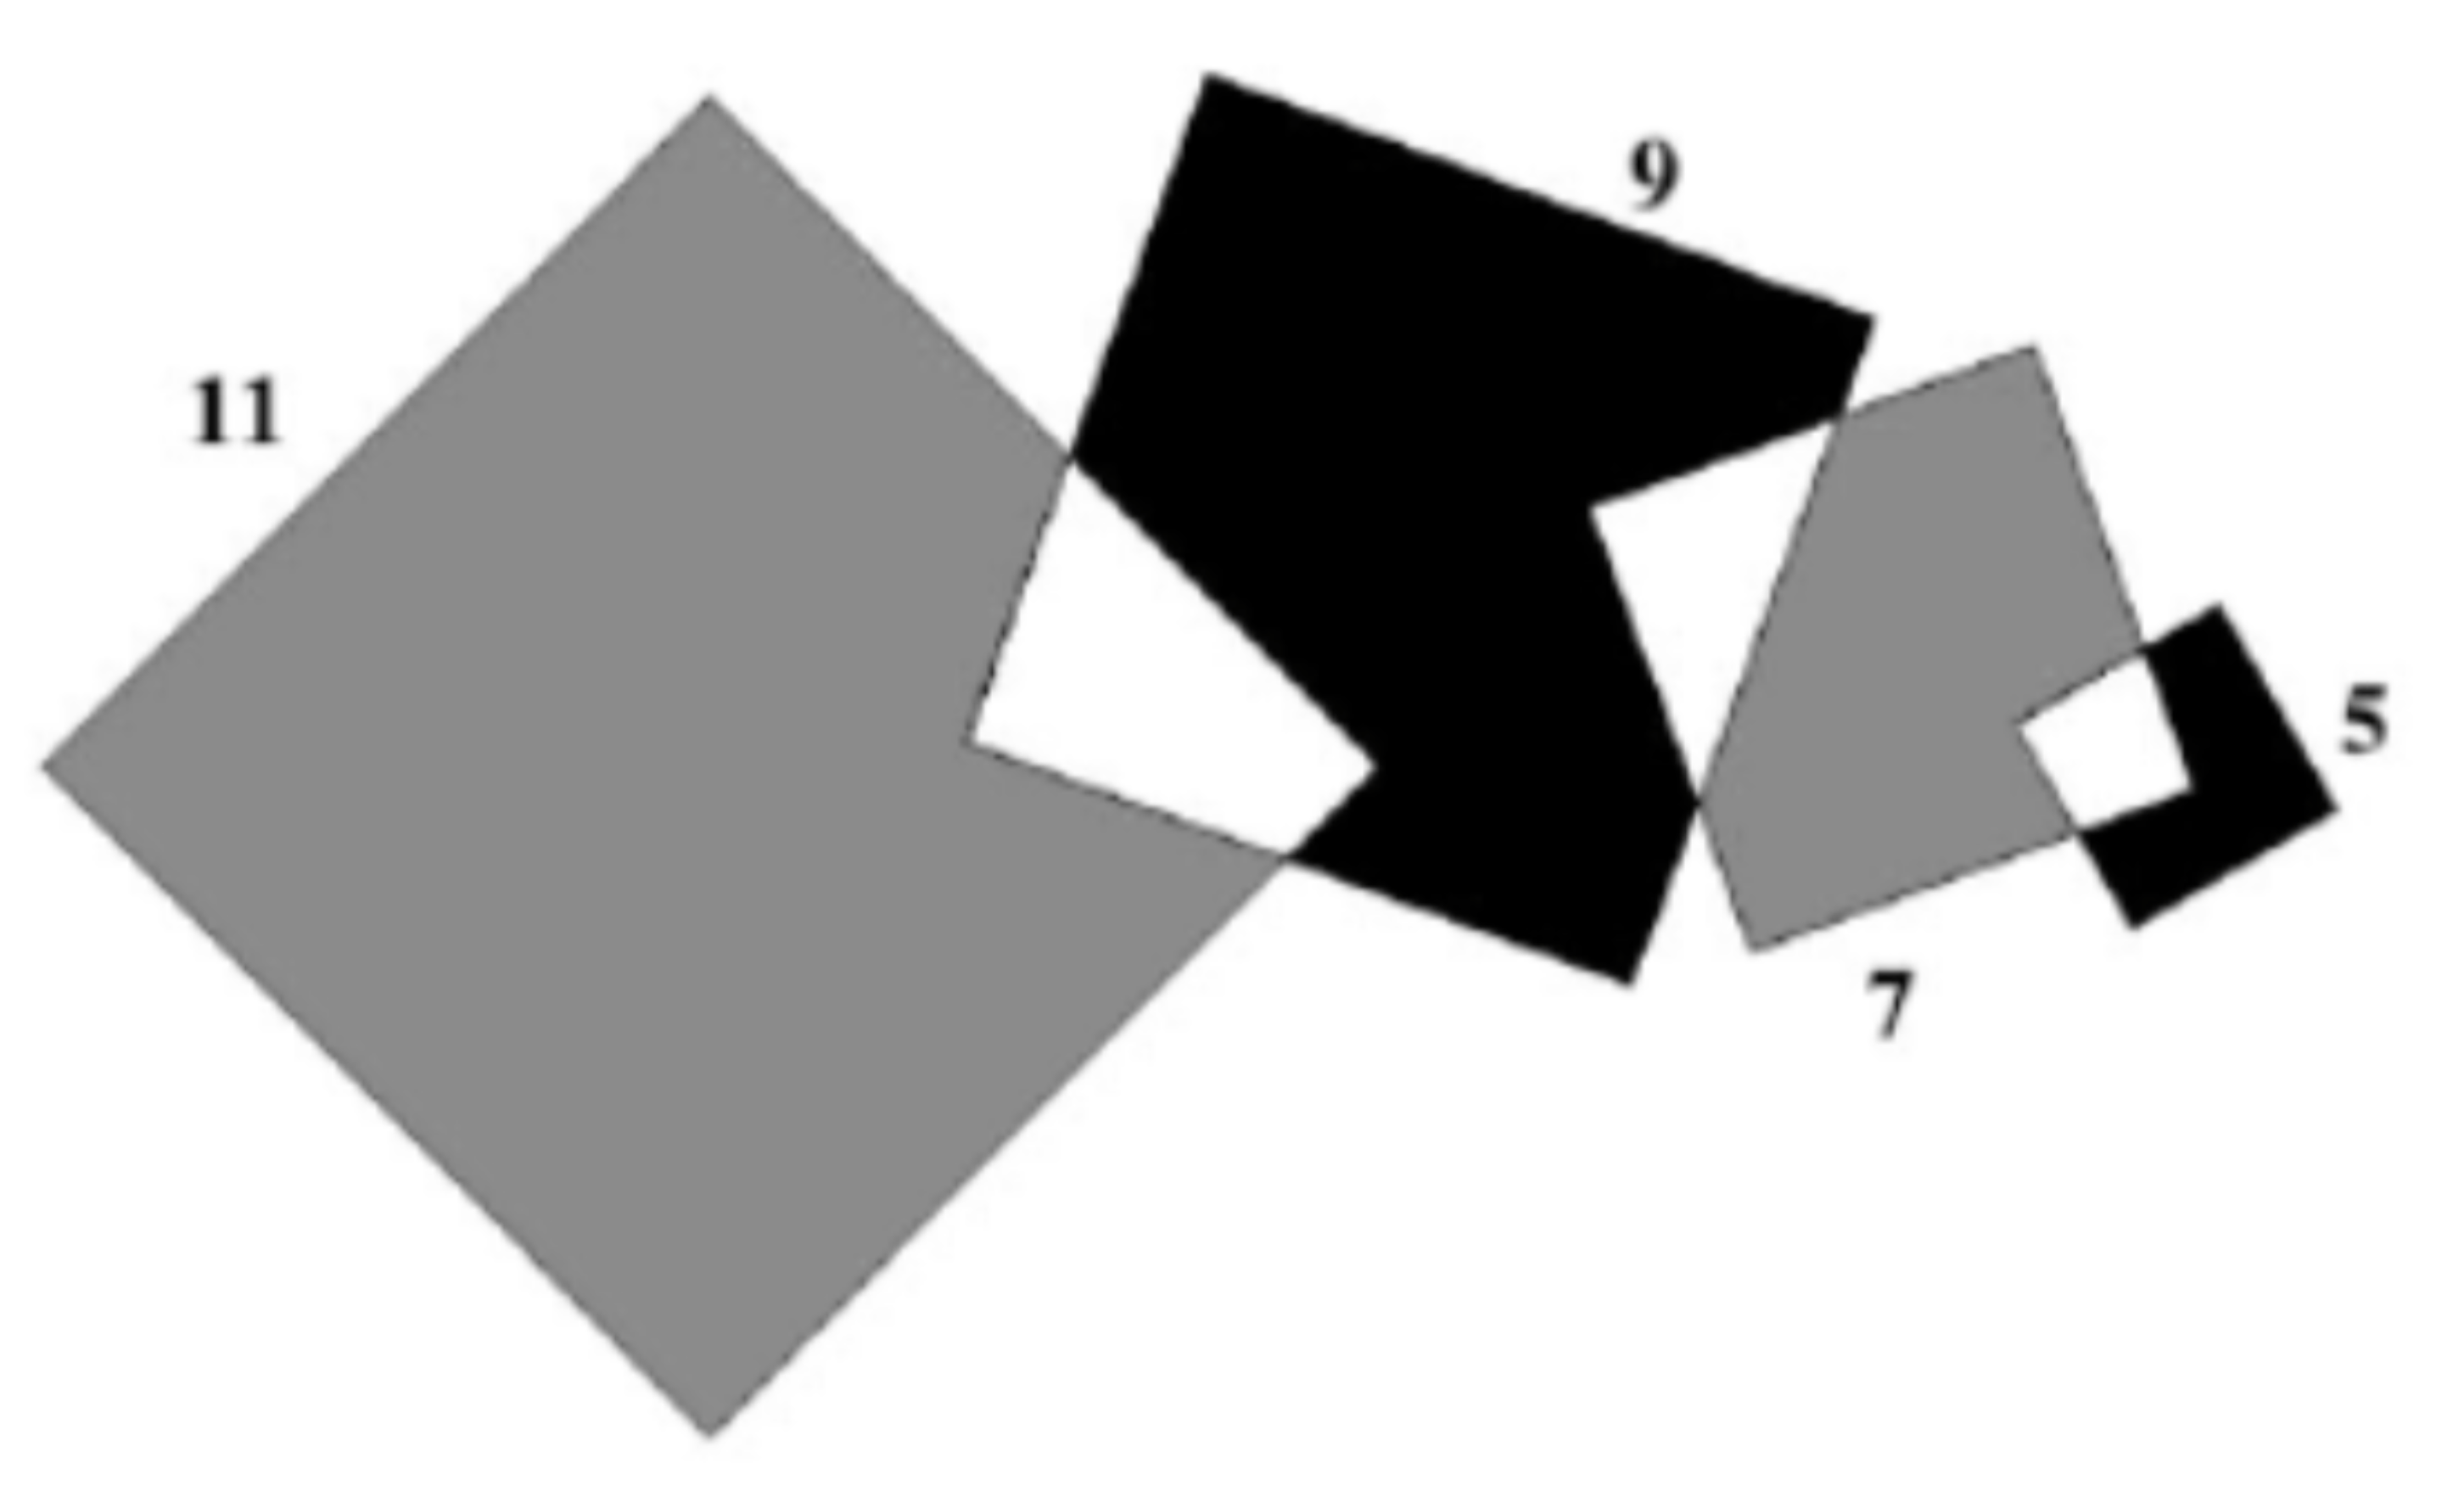
\includegraphics[width=0.5\textwidth]{squares.png}
\end{figure}

The gray surface is twice as large as the black surface. What is the area of the white surface?



\section{2024-06-27: Digit sum times 2024}

Let $Q(n)$ be the sum of digits of a natural number $n$. For all $n$, $Q(2n) \leq 2Q(n)$.

Find a number $n$ such that $Q(n) = 2024 \cdot Q(3n)$.

\vspace{1em}

Restating the problem, we know that for all $n$:
\[ \frac{Q(2n)}{Q(n)} \leq 2 \]
and we want some $n$ such that:
\[ \frac{Q(3n)}{Q(n)} = \frac{1}{2024} \leq 2 \]

Let's use the notation $x\{k\}y$ to denote a natural number in base 10 where the digit $x$ is repeated $k$ times
and followed by the digit $y$.

Playing around a bit to build intuition, for all positive $k$, $2(9\{k\}9) = 19\{k\}8$ and
\[ \frac{Q(19\{k\}8)}{Q(9\{k\}9)} = \frac{1+9k+8}{9k+9} = 1\]

Similarly, $2(1\{k\}) = 2\{k\}$ and
\[ \frac{Q(2\{k\})}{Q(1\{k\})} = 2\]

Intuitively, we want to find some increasing sequence of numbers $n_i$ that contain a repeating pattern of digits
such that $Q(n_i)$ grows much more quickly than $Q(3n_i)$ as the pattern of digits increases in length.
Can we find a $3n$ that consists mostly of 0s while $n$ does not?

The simplest pattern for which this is true is numbers of the form $n = 3\{k\}y$ with $y \in \{ 4, 5, 6 \}$. Then
$3n = 10\{k\}z$, where $z \in \{ 2, 5, 8 \}$, respectively.

We may be onto something! Let's build a table:

\begin{table}[h!]
\centering
\begin{tabular}{|c|c|c|c|}
	\hline
	$n$      & $3\{k\}4$    & $3\{k\}5$    & $3\{k\}6$ \\
	\hline
	$3n$     & $10\{k\}2$   & $10\{k\}5$   & $10\{k\}8$ \\
	\hline
	$Q(n)$   & $3k+4$       & $3k+5$       & $3k+6$ \\
	\hline
	$Q(3n)$  & $3$          & $6$          & $9$ \\
	\hline
\end{tabular}
\end{table}

$\frac{3k+4}{3} = 2024$ has no integer solution (for any $m$, $3m-4 \mod 3 = 2$).

$\frac{3k+5}{6} = 2024$ has no integer solution (for any $m$, $6m-5 \mod 3 = 1$).

But $\frac{3k+6}{9} = 2024$ does have an integer solution ($9m-6 \mod 3 = 0$). $k = 6070$,
so $n = 3\{6070\}6$ (and $3n = 10\{6070\}8$).


\end{document}  